\documentclass[10pt,a4paper,oneside,openany,noindent]{book}
\usepackage[utf8]{inputenc}

\usepackage{amsmath}

\usepackage{amsfonts}
\usepackage{amssymb}
\usepackage{graphicx}
\setlength\parindent{0pt}
\usepackage[pagestyles]{titlesec}
%\titleformat{\chapter}[display]{\normalfont\bfseries}{}{0pt}{\Huge}
\newpagestyle{mystyle}
{\sethead[\thepage][][\chaptertitle]{}{}{\thepage}}
\pagestyle{mystyle}
\usepackage{algorithm}
\usepackage{algpseudocode}
\newcommand{\ph}{\hat{p}}
\newcommand{\direct}{x'|x}
\newcommand{\inverse}{x|x'}
\newcommand{\normal}[2]{\mathcal{N}\left(#1,#2\right)}
\newcommand{\pk}{\textbf{P}_k}
\newcommand{\pknew}{\textbf{P}_{k'}}
\newcommand{\eq}{\textbf{E}_q}
\newcommand{\eqnew}{\textbf{E}_{q'}}
\newcommand{\ak}{\textbf{a}_k}
\newcommand{\aknew}{\textbf{a}_{k'}}
\newcommand{\y}{\textbf{y}}
\newcommand{\bq}{\textbf{b}_q}
\newcommand{\bqnew}{\textbf{b}_{q'}}
\renewcommand{\eq}{\textbf{E}_q}
\newcommand{\ve}{\sigma_e^2}
\newcommand{\va}{\sigma_a^2}
\newcommand{\vb}{\sigma_b^2}
\newcommand{\la}{\lambda_a}
\newcommand{\lb}{\lambda_b}
\newcommand{\unif}{\mathcal{U}[0,1]}

\begin{document}
\chapter{Introduzione}
\begin{minipage}{0.5\textwidth}
\noindent
The number of things you don't know is one of the things you don't know\vspace{1em}\\Peter Green
\end{minipage}\vspace{3em}\\
Quando si vuole identificare un sistema dinamico bisogna
\begin{itemize}
\item stabilire la struttura del legge dinamica
\item stabilire il valore numerico delle costanti del modello
\end{itemize}
La prima richiesta consiste nel decidere il tipo e il numero di operazioni sui segnali di ingresso e di stato che sono in grado di riprodurre accettabilmente ( e possibilmente con una legge compatta) la dinamica del sistema.
La seconda richiesta consiste invece nel determinare il valore numerico dei parametri che intervengono.\\


I casi in cui è sufficiente una identificazione parametrica sono i casi in cui si ha già la struttura della legge. Per ottenere la legge (a meno del valore delle costanti) è necessario uno studio del sistema a partire dai principi primi che regolano tutti i fenomeni che sono coinvolti. In definitiva l'idengtificazione parametrica è sufficiente solo se sono verificate le seguenti condizioni
\begin{itemize}
\item è \textbf{possibile} ottenere una descrizione del sistema applicando i principi primi delle scienze
\item è \textbf{vantaggioso} ottenere una descrizione del sistema applicando i principi primi delle scienze (tempo speso, rischio di errori etc)
\item ci si accontenta della descrizione ottenuta applicando i principi primi delle scienze (rischio di tralasciare fenomeni importanti)
\item la complessità delle leggi che si ottengono applicando i principi primi delle scienze non è tale da renderle inutilizzabili
\end{itemize}

Quando una di queste condizioni non è soddisfatta è possibile inserire nel processo di identificazione anche la ricerca della struttura del modello.
A tale scopo si ipotizza una classe (abbastanza vasta) di strutture di modello
e si lascia al processo di identificazione l’onere di scegliere quella che maggiormente si adatta
alle misure. I metodi Bayesiani in particolare sono appropriati per la selezione dei
modelli perchè forniscono naturalmente (senza analisi aggiuntve) un contesto in cui
si quantifica l’incertezza associata all’identificazione. L’approccio bayesiano infatti, non fornisce una singola descrizione del sistema ma fornisce una distribuzione di
probabilità associata al set di modelli possibili. Dunque risolvere il problema di
inferenza bayesiana conduce a scelte più  ponderate rispetto alla semplice estrazione
del modello che si adatta meglio ai dati reali. Analizzando la distribuzione prodotta
si può per esempio individuare un modello poco meno accurato del migliore ma
preferirlo perchè meno complesso .\\
Nella seguente trattazione la classe di modelli scelta è quella dei nonlineari, auto-regressivi, a media mobile
con ingressi esogeni (NARMAX); essa è una popolare classe modelli ingresso-uscita
spesso usata nell’identificazione di sistemi non lineari in vari ambiti dell’ingegneria
(e non) poichè ha il pregio di produrre leggi compatte ma accurate.
Come si vedrà nei successivi capitoli, ciascun modello NARMAX può essere visto
come lo sviluppo su una opportuna base polinomiale della legge che
regola il sistema. Ciò che distingue un modello da un altro è il numero e l’insieme
dei termini presenti nello sviluppo.

La ricerca esaustiva tra tutte le possibili combinazioni di termini NARMAX è tuttavia quasi sempre computazionalmente improponibile , così si è puntato negli ultimi
anni a sviluppare metodi di campionamento efficaci che, avvalendosi di una catena
di Markov opportunamente costruita, esplorano in maniera non esaustiva l’insieme
dei modelli ottenendo comunque statistiche significative.
\chapter{Identificazione bayesiana e metodi
di campionamento Monte Carlo}
\section{Approccio Bayesiano per l’identificazione}
L’inferenza bayesiana è un approccio all’inferenza statistica in cui le probabilità
non sono interpretate come frequenze ma piuttosto come livelli di fiducia nel verificarsi di un dato evento. Il nome deriva dal teorema di Bayes, che costituisce il
fondamento di questo approccio. Gli statistici bayesiani sostengono che i metodi
dell’inferenza bayesiana rappresentano una formalizzazione del metodo scientifico,
che normalmente implica la raccolta di dati che avvalorano o confutano una data
ipotesi.
Queste caratteristiche rendono l’approccio bayesiano un utile ausilio per discriminare tra alternative in conflitto e dunque un ottimo strumento per l’identificazione
dei sistemi.
Il metodo usa una stima del grado di fiducia in una data ipotesi prima dell’osservazione
dei dati al fine di associare un valore numerico al grado di fiducia in quella stessa
ipotesi successivamente all’osservazione dei dati. Si supponga di voler identificare
un sistema scegliendo il più adatto in un insieme M di modelli.
Sia M una variabile aleatoria che rappresenta la legge che regola il vero sistema.
L’obiettivo dell’identificazione bayesiana è quello di calcolare per ogni $m\in M$ la
probabilità a posteriori
\begin{equation} P (M = m|Y )
\end{equation}
dunque complessivamente determinare la distribuzione della probabilità sull’insieme
dei modelli condizionatamente alle misure.
La probabilità condizionata è stata definita in termini della probabilità congiunta e
marginale dei due eventi
\begin{equation}
P (M = m|Y ) =
P (M = m, Y )
P (Y )
\end{equation}

la definizione corrisponde all’idea ragionevole
\begin{equation}
P (M = m|Y ) \propto P (M = m, Y )
\end{equation}

Avendo però ristretto l’insieme di supporto su cui è definita la metrica di probabilità,
è necessario imporre che valgano ancora gli assiomi della probabilità, in particolare
chiamando k la costante di proporzionalità e integrando su tutti i casi possibili si ha
\begin{equation}P (M = m|Y )dm =
k \cdot P (M = m, Y )dm = k \cdot P (Y ) := 1\end{equation}
da cui si ricava il valore di k
\begin{equation}k =
\frac{1}{P(Y)}
\end{equation}
ottenendo la definizione di probabilità condizionata.
Scambiando i ruoli delle variabili aleatorie si ha anche che
\begin{equation}
P (Y |M = m) =
P (M = m, Y )
P (M = m)
\end{equation}


dunque mettendo insieme le equazioni [EQUAZIONI] si ottiene la formula di Bayes
\begin{equation}
P (M = m|Y ) =\frac{
P (Y |M = m)P (M = m)}{
P (Y )}
\end{equation}

usando il teorema della probabilità totale si pu`o inoltre esprimere la costante al
denominatore in funzione delle quantità al numeratore ottenendo
\begin{equation}
P (M = m|Y ) =\frac{
P (Y |M = m)P (M = m)}{\int
P (Y |M = m)P (M = m)dm}
\end{equation}
Nei problemi di identificazione l’espressione della probabilità a posteriori è quasi
sempre impossibile da valutare analiticamente sopratutto per colpa dell’integrale al
denominatore che deve essere calcolato su tutti i possibili modelli; si ricorre quindi a
metodi numerici di tipo Monte Carlo basati sul campionamento della distribuzione.
Spesso risulta impossibile anche campionare direttamente la distribuzione e se ne
deve ottenere una stima accettando o scartando opportunamente i campioni estratti
da una distribuzione più semplice.
\section{Idea dei metodi Monte Carlo}
I metodi Monte Carlo sfruttano il seguente ragionamento: se si vuole  campionare una distribuzione con densità $p(x)$ (nel nostro caso la posterior sui modelli) si ha
\begin{equation}
p(x)=p(x)\otimes \delta(x)=\int_\xi p(\xi)\delta(x-\xi)d\xi
\end{equation}
se poi $p(x)$ è fattorizzabile come \begin{equation}
p(x)=q(x)g(x)
\end{equation}
tale che $q(x)$ sia una densità di probabilità ovvero
\begin{itemize}
\item $q(x)>0$ per ogni $m$
\item $\int_m q(x)=1$
\end{itemize} allora
\begin{equation}
p(x)=\int_\xi q(\xi)g(\xi)\delta(x-\xi)= E[g(Q)\delta(x-Q)]
\end{equation}
con $Q$ variabile aleatoria avente come densità $q(\cdot)$.
Usando uno stimatore si può approssimare il valore atteso come
\begin{equation}
E[g(Q)\delta(x-Q)]\simeq \frac{1}{N}\sum_{k=1}^N g(q_k)\delta(x-q_k)
\end{equation}
con $q_k\sim q(\cdot)$ campione estratto dalla distribuzione di densità di proposal $q(\cdot)$
In pratica si estraggono numerosi modelli da una distribuzione di proposal $q(\cdot)$,
e si costruisce un istogramma pesato con i pesi 
\begin{equation}
g(q_k)=\frac{p(q_k)}{q(q_k)}
\end{equation}
Si noti che nella formula dei pesi la desnsità  $p(\cdot)$ è solamente una funzione da valutare in uno specifico modello, cosa che quasi sempre è fattibile  perchè richiede una informazione che è locale nello spazio dei modelli, al contrario del problema di campionare direttamente la densità che richiederebbe una conoscenza della funzione su tutto lo spazio.\\
\section{Importance sampling: scelta della proposal}
In teoria le precedenti considerazioni sono già sufficienti per campionare la distribuzione, in pratica la scelta di una proposal opportuna è critica per l'accuratezza dell'algoritmo. Nella realtà, avendo a disposizione un tempo limitato, e quindi un numero limitato di campionisi otterrà una approssimazione della distribuzione cercata.
La proposal è determinante nell'imporre alcuni criteri di approssimazione\\
Partendo dal presupposto ovvio che non è possibile esplorare esaustivamente lo spazio dei modelli, bisogna fare delle assuzioni su quali regioni dello spazio dei modelli esplorare maggiormente (e quindi descrivere) e quali invece trascurare.\\
E' sensato disinteressarci delle regioni in cui i modelli hanno bassa probabilità.
Ai fini dell'identificazione, non ci interesserà mai confrontare due modelli con probabilità bassa. Si può benissimo sbagliare o ignorare il rapporto reciproco tra le loro probabilità per concentrarsi sulla descrizione delle regioni dove i modelli hanno probabilità più alta.
Questo induce a scegliere la proposal quanto più simile alla posterior, in modo da estrarre campioni prevalentemente dove la posterior è alta.
Tale criterio è detto di \emph{importance sampling}.\\ \\
Al limite se riuscissi ad essere sicuro che sto campionando da $q(\cdot)=p(\cdot)$ 
avrei che i pesi si ridurrebbero a
\begin{equation}
g(q_k)=\frac{p(q_k)}{q(q_k)}=\frac{p(q_k)}{p(q_k)}=1
\end{equation}
e dunque
\begin{equation}
p(x)\simeq \frac{1}{N}\sum_{k=1}^N \delta(x-q_k)
\end{equation}
Ovvero potrei avere una approssimazione di $p(\cdot)$ semplicemente valutando la frequenza relativa con cui è stato estratto $q_k=x$.
Attenzione, l'ipotesi di sapere che $q(\cdot)=p(\cdot)$ non vuol dire che conosco la forma della funzione su tutto lo spazio, ma solo che
\begin{itemize}
\item so valutare la funzione in un particolare modello
\item ho un metodo (anche indiretto) per campionare la funzione
\end{itemize}

Gli algoritmi Monte Carlo Markov Chain infatti ottengono i modelli $q_k$ 
come stati di una catena di Markov opportunamente costruita sullo spazio dei modelli. A tale catena si chiede di avere come unica probabilità di regime proprio $p(\cdot)$.\\
Dopo un transitorio iniziale la catena finirà di fatti per campionare i suoi stati dalla distribuzione di regime $p(\cdot)$.
\chapter{Algoritmo Metropolis Hasting}
Supponiamo di voler estrarre campioni da una distribuzione p(m) nota, difficile da
campionare direttamente.
Si pu`o chiedere che la distribuzione obiettivo sia
distribuzione di regime di una catena di Markov. Una catena si dice ergodica se
dopo un certo tempo (transitorio iniziale) , essa converge all'unica distribuzione
di regime indipendentemente dalla distribuzione di partenza.
Le condizioni necessarie per l’ergodicit`a della catena sono:
\begin{itemize}
\item \textbf{irriducibilit`} : la probabilit`a di visitare ciascuno stato a partire da ciascuno
stato `e strettamente positiva
\item \textbf{aperiodicità} : una catena `e periodica se pu`o ritornare in un certo stato solo
a istanti multipli di un qualche intero maggiore di 1. Una catena `e aperiodica
se non `e periodica.
\end{itemize}

In poche parole, fissato un qualsiasi istante abbastanza grande e un qualsiasi stato,
deve essere possibile una storia temporale della catena che la porta a risiedere in
quello stato a quell’istante. La questione diventa quindi come scegliere il kernel
\begin{equation*}
s(x' |x) 
\end{equation*}
(probabilit`a di transizione dal vecchio stato m al nuovo stato m' ) della catena,
in modo che la catena sia ergodica e che la distribuzione di regime sia proprio p(m).
Una condizione sufficiente non necessaria `e che la distribuzione obiettivo soddisfi la
condizione di reversibilit`a

\begin{equation}
p(x)s(x' |x) = p(x')s(x|x' )
\end{equation}

L'operatore di transizione è quello che nelle catene a stato discreto e finito era rappresentato dalla matrice di transizione mentre nelle catene a stato continuo è il funzionale
\begin{equation}
Tr[\bullet]=\int \bullet(x)s(x'|x)dx
\end{equation}
Una  densit`a di probabilit`a $\ph$ `e detta stazionaria se `e autofunzione
dell’operatore di transizione della catena, ovvero\\
\begin{equation}
Tr[\ph]=\ph
\end{equation}
e semplice dimostrare che se vale la condizione di reversibilit`a allora la distribuzione
`e stazionaria infatti
\begin{equation*}
\begin{split}
Tr[\ph]=\int \ph(x)s(x'|x)dx=\int \ph(x')s(x|x')dx=\\
\ph(x')\int s(x|x')dx=\ph(x')\cdot 1=\ph(x')
\end{split}
\end{equation*}

Se si sceglie un kernel arbitrario uguale ad una probabilit`a di transizione facile
da campionare $s(\direct) = q(\direct) $ solitamente la condizione di reversibilit`a non `e
soddisfatta. Solitamente si ha uno sbilanciamento che significa che alcune transizioni
sono pi`u probabili in un certo verso.
\begin{equation}
\ph(x)s(\direct)>\ph(x')s(\inverse)
\end{equation}

In tal caso, viste le distribuzioni di partenza e la probabilit`a di transizione scelta `e
pi`u probabile osservare la transizione $x\rightarrow x'$ piuttosto che la transizione $x'\rightarrow x$
Si cerca quindi di ristabilire l’equilibrio scegliendo come kernel la probabilit`a di
transizione moltiplicata per un fattore correttivo 
\begin{equation}
q(\direct) = \gamma(\direct)q(\direct)
\end{equation}
In particolare si pu`o interpretare $\gamma(\direct)$ come la probabilit`a di accettare la mossa $x \rightarrow x'$. Imponendo quindi che valga


\begin{equation}
\ph(x)\gamma(\direct)q(\direct)=\ph(x')\gamma(\inverse)q(\inverse)
\end{equation}
si ricava
\begin{equation}
\frac{\gamma(\direct)}{\gamma(\inverse)}=\frac{\ph(x')q(\inverse)}{\ph(x)q(\direct)}
\end{equation}

Perch`e si abbia coerenza con la eq[CITARE EQUAZIONE] bisogna che il rapporto al membro sinistro sia minore di 1. In particolare si può scegliere

\begin{itemize}
\item $\gamma(\inverse)=1$ che equivale ad accettare tutte le transizioni $m' \rightarrow m$ che sono meno
frequenti
\item $\gamma(\direct)=min\left\lbrace 1,\frac{\ph(x')q(\inverse)}{\ph(x)q(\direct)}\right\rbrace$ fattore di riduzione delle transizioni pi`u frequenti
\end{itemize}
 L'algoritmo MH è così definito  \\
\hrule 
\textbf{Algoritmo} Metropolis Hastings
\hrule
\begin{algorithmic}
\State Inizializza  $X_0=x_0$
\For {$t=0,1,2\dots T$}
    \State $i\gets 0$

\State Estraggo la proposta per il nuovo stato $x^t \sim q(x^t |X_t)$
\State Calcolo la probabilità di accettare la mossa $\gamma(\direct)=min\left\lbrace 1,\frac{\ph(x^t)q(X_t | x^t)}{\ph(X_t)q(x^t|X_t  )}\right\rbrace$
\State Estraggo una variabile da una distribuzione uniforme $u\sim U(0,1)$
\If {$u \leq \gamma(x^t | X_t)$}
 \State La catena transita nel nuovo stato proposto $X_{t+1}=x^t$
\Else
\State La catena rimane nel vecchio stato $X_{t+1}=X_t$
\EndIf
\EndFor
\end{algorithmic}


\chapter{Reversible Jump Monte Carlo Markov Chain}
Nelle sezioni precedenti la transizione della catena associava (in maniera aleatoria)
uno stato di $X\subset \mathbb{R}^n$ ad uno stato di  $X'\subset \mathbb{R}^n$ .
Cosa succede se la transizione dovesse associare uno stato $M\subset \mathbb{R}^n$ ad uno stato
di $X\subset \mathbb{R}^m$ con $ m = n$?
La questione scaturisce dal fatto che per gli scopi dell’identificazione dei sistemi,
restringersi al caso $m = n$ `e molto limitativo e corrisponde a conoscere in partenza
il numero dei parametri da identificare.
Per i sistemi non lineari spesso si considerano modelli del sistema che sono sviluppi
polinomiali di equazioni alle differenze e si lascia all’algoritmo di identificazione
l’onere di determinare quali e quanti termini dello sviluppo includere.
In base al numero di termini scelti si avranno da scegliere anche altrettanti coeffici-
enti dello sviluppo.
Quando l’algoritmo suggerisca di aggiungere o eliminare uno (o pi`u) termini dello
sviluppo `e necessario aggiornare anche la dimensione del vettore dei coefficienti.
Ecco quindi che acquistano senso mosse che portano lo stato della catena da uno
spazio con una certa dimensionalit`a ad un’altro con dimensionalit`a diversa.
Si pensi quindi di enumerare le tipologie di modello (anche infinite), si avr`a che
l’insieme delle possibili strutture di modello `e rappresentabile come un insieme di
indici
\begin{equation*}
\mathcal{K}=\left\lbrace 1,2,\dots k \dots\right\rbrace \subset \mathbb{N}
\end{equation*}
Ciascun modello `e associato uno spazio dei coefficienti dello sviluppo ( o in generale
dei parametri del modello).
Si ha quindi che a ciascuna tipologia di modello `e associato uno spazio 
\begin{equation*}
X_k\subset\mathbb{R}^{n(k)}
\end{equation*} 
dove $n(k)$ `e il numero di termini previsti dal modello indicizzato da $k$.
Si pu`o quindi pensare che la ricerca del modello avvenga in una unione di sottospazi
definita da
\begin{equation}
X=\bigcup_{k\in \mathcal{K}}(\{k\}\times X_k)
\end{equation}

L’inclusione esplicita dell’indice k si ha perch`e spesso `e necessario che l’algoritmo vi
acceda, specialmente quando esistono pi`
u modelli diversi a cui corrisponde lo stesso
spazio dei parametri.
Lo stato della catena `e quindi rappresentabile come coppia $x = (k, \theta_k )$ dove k indica
l’indice della struttura di modello e $\theta_k$ indica i parametri associati a tale struttura,
il numero di parametri dipende da k.
Se pur lo spazio appena costruito sia un po’ inusuale, l’algoritmo MH `e ancora
valido, si tratta di vedere come costruire una catena di Markov che abbia lo stato
in questo insieme X e che abbia una desiderata densit`a di regime $\ph(\cdot)$ .\\
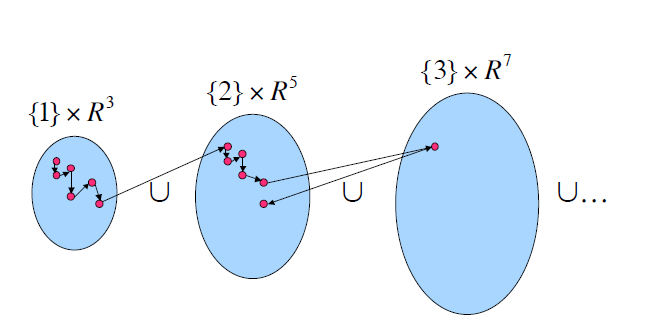
\includegraphics[width=0.8\textwidth]{RJMCMCImage.png}\\ 
Ci limitiamo a considerare i casi in cui, per qualche distribuzione di probabilit`a di
partenza la probabilit`a che la catena risieda in un sottoinsieme $A \subset X$ e muova
verso un certo $B\subset X$ sia la stessa qualora si scambino i ruoli di A e di B. Questa
richiesta `e detta di equilibrio bilanciato , se verificata da una certa probabilit`a `e una
condizione sufficiente affinch`e questa sia stazionaria.

Spesso per attraversare lo spazio X `e necessario avere a disposizione diverse tipolo-
gie di mosse.
Una tipologia di mossa associa la struttura del modello attuale ad una nuova strut-
tura.
Affinch`e la condizione di equilibrio bilanciato sia soddisfatta `e necessario che se es-
iste la mossa $( x \rightarrow x' )$ esista anche la mossa inversa $(x' \rightarrow x)$ .
Si indichi con $j_m (x)$ la probabilit`a che dallo stato x sia scelta la mossa di tipo m e
si indichi con $j_m^{-1}
(x ) $la probabilit`a che dallo stato x sia scelta la mossa di tipo m
inversa.
Il problema `e che non ha senso paragonare probabilit`a definite su spazi di dimen-
sione diversa.
Per rendere invisibile alla catena il cambio di dimensionalit`a basta immergere i due
spazi di dimensione diversa in uno stesso spazio di dimensione maggiore e definire
in tale spazio la probabilit`a.
Si adotti quindi il seguente protocollo (ideato da Peter Green nel 1995):
\begin{itemize}
\item Si estragga la tipologia di mossa.
\item Si generino r numeri casuali $u\in\mathbb{R}^r$ da una specificata densit`a g.
\item Si costruisca il nuovo stato attraverso una funzione deterministica h di x e di u.
\begin{equation}
(x' , u' ) = h(x, u)
\end{equation}
In questo caso sono stati indicati con u gli r numeri che sono estratti casualmente
dalla distribuzione g quando si effettua la mossa inversa da x' a x usando la funzione
deterministica inversa
\begin{equation}
(x, u) = h ^{-1}(x' , u ')
\end{equation}
l’equazione di equilibrio bilanciato si pu`o scrivere dunque come
\begin{equation*}
\sum_m \int_{(x,x')\in A\times B}j_m(x)\ph(x)g_m(u)\gamma_m(x'|x)dxdu=
\sum_m \int_{(x,x')\in A\times B}j_m^{-1}(x')\ph(x')g_m(u')\gamma_m(x'|x)dx'du'
\end{equation*}
La sommatoria sulle possibili mosse deriva dal fatto che ad ogni iterazione la tipolo-
gia di mossa `e esclusiva. Una condizione sufficiente non necessaria perch`e valga il
bilancio `e che esso valga mossa per mossa ovvero
\end{itemize}
\begin{equation*}
 \int_{(x,x')\in A\times B}j_m(x)\ph(x)g_m(u)\gamma_m(x'|x)dxdu=
 \int_{(x,x')\in A\times B}j_m^{-1}(x')\ph(x')g_m(u')\gamma_m(x'|x)dx'du'
\end{equation*}
se inoltre la funzione h `e un diffeomorfismo vale la formula classica del cambio
di variabili e quindi si pu`o passare dall’uguaglianza integrale all’uguaglianza delle
integrande.
Dal momento che la mossa `e fissata si ha che k e k' sono costanti dunque il cambio
di variabili richiesto riguarda solo il vettore dei parametri e delle variabili ausiliarie.
\begin{equation*}
(\theta_k',u')\rightarrow(\theta_k,u)
\end{equation*}
Applicandolo si ottiene
\begin{equation*}
j_m(x)\ph(x)g_m(u)\gamma_m(x'|x)=
j_m^{-1}(x')\ph(x')g_m(u')\gamma_m(x'|x)\left\vert\frac{\partial(\theta_{k'},u') }{\partial(\theta_{k},u) }\right\vert
\end{equation*}
Condizione necessaria affinch`e h sia un diffeomorfismo `e che
\begin{equation}
dim(\theta_{k'})+dim(u')=dim(\theta_{k})+dim(u)
\end{equation}
detta condizione di \emph{dimension matching}. Si ha dunque in tal caso che
\begin{equation}
\gamma_m(x'|x)=\min\left\lbrace 1,\frac{
j_m^{-1}(x')\ph(x')g_m(u')\gamma_m(x'|x)}
{j_m(x)\ph(x)g_m(u)}
\left\vert\frac{\partial(\theta_{k'},u') }{\partial(\theta_{k},u) }\right\vert 
\right\rbrace
\end{equation}
\end{document}
